\documentclass{article}
\usepackage{color}
\usepackage{graphicx}
\usepackage{setspace}

\usepackage{geometry}
\usepackage{amsmath}
\usepackage{enumitem,amssymb}
\usepackage{pifont}
\definecolor{darkgreen}{rgb}{0.0, 0.5, 0.0}
\geometry{left = 1.25in, right=1.25in} % New Stuff Learned!
\newcommand{\cmark}{\ding{51}}
\newcommand{\xmark}{\ding{55}}
\newcommand{\done}{\rlap{$\square$}{\raisebox{2pt}{\large\hspace{1pt}\cmark}}
\hspace{-2.5pt}}
\newcommand{\wontfix}{\rlap{$\square$}{\large\hspace{1pt}\xmark}}
\newlist{todolist}{itemize}{2}
\setlist[todolist]{label=$\square$}
\doublespacing
\begin{document}
\begin{titlepage}
	

\title{\textbf{ECE358 Week 1}}
\author{\textit{Sanzhe Feng}}
\date{\textit{\today}}
\maketitle
\end{titlepage}
\setlength{\parindent}{0pt}

\textbf{\emph{Asmptotic}} efficiency of algorithms decribes when the size of the input increases without bound.

\section*{3.1 Asymptotic Notation}

\subsection*{Asymptotic notation, functions, and running times}
Asymptotic notation actually applies to functions. For example, the worst-case running time for insertion sort is $an^2+bn+c$, but when we write the asymptotic notation as $\Theta(n^2)$.
\subsection*{$\Theta$-notation}
Definition: For given function $g(n)$, a function $f(n)$ belongs to the \textbf{set} $\Theta(g(n))$ if there exists positive constants $c_1$, $c_2$ and $n_0$ such that $0 \leq c_1g(n)\leq f(n)\leq c_2g(n)$ for all $n \geq n_0$.

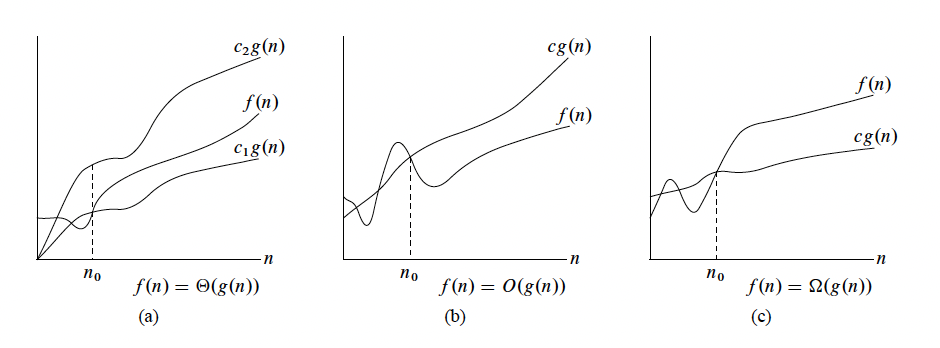
\includegraphics[width=1\linewidth]{P45_3.1.png}
\begin{center}
\small{Figure 1.1 Graphic examples of the $\Theta,$ $\Omega$ and $O$ notations (CLRS P45)}	
\end{center}

Such relationship can be expressed by $f(n) \in \Theta(g(n))$ or $f(n) = \Theta(g(n))$, and $g(n)$ is the \textbf{\textit{asymptotically tight bound}} for $f(n)$. This definition requires that $f(n)$ is nonnegative whenever n is sufficiently large (\emph{\textbf{asymptotically nonnegative}}). Consequently, $g(n)$ needs to be the same way. \\


A formal justification of  $f(n) = \Theta (n)$ where $f(n) = an^2+bn+c$ where $a,b,c$ are constants and $a > 0$. We can easily pick $c_1 = a/4, c_2 = 7a/4$ and $n_0 = 2 \cdot max(|b|/a, \sqrt{|c|/a})$ and verify that 
$0 \leq c_1n^2\leq an^2+bn+c\leq c_2n^2$ (definition). The important thing is that \textbf{some choice exists}. In general, for any polynomial $p(n)=\sum_{i=0}^{k}a_in^i$, we have $p(n) =\Theta(n^d)$ when $a_i$ are constants and $a_d>0$. We can also express constant functions as $\Theta(n^0)$ or $\Theta(1)$.

\subsection*{O-notation}

\textbf{Asymptotic upper bound}. 
Definition: For given function $g(n)$, a function $f(n)$ belongs to the \textbf{set} $O(g(n))$ if there exists positive constants $c$ and $n_0$ such that $0 \leq f(n)\leq cg(n)$ for all $n \geq n_0$. Note that $f(n) = \Theta(g(n))$ \textbf{implies} $f(n) = O(g(n))$ and $f(n) = \Omega(g(n))$. Therefore, if $\Theta (n^2)$, then $O(n^2)$.\\

Suprisingly,we found any linear function $an+b, a>0$ is in $O(n^2)$. This is because in this book, we do not claim about \textbf{HOW TIGHT AN UPPER BOUND IS}. \\

$O$-notation describes an upper bound, when we use it to bound the worstcase
running time of an algorithm, we have a bound on the running time of the algorithm
on \textbf{every input}. Thus, the $O(n^2)$
bound on \textbf{worst-case running time of insertion sort also applies to its running time
on every input}. The $\Theta(n^2)$ bound on the worst-case running time of insertion sort,
however, does not imply $\Theta(n^2)$ bound on the running time of insertion sort on
every input. Since there is an input that makes insertion sort runs in $\Theta(n)$ time. (The simple $\Theta(n^2) \neq \Theta(n^2)$ idea).\\

When we say the running time of insertion sort is $O(n^2)$, we MEAN no matter what the input is, the time is bounded from above by $f(n)$.


\subsection*{$\Omega$-notation}
\textbf{Asymptotic lower bound}. 
Definition: For given function $g(n)$, a function $f(n)$ belongs to the \textbf{set} $\Omega(g(n))$ if there exists positive constants $c$ and $n_0$ such that $0 \leq cg(n) \leq f(n)$ for all $n \geq n_0$.\\

 Based on these three definitions, we can have the following theorem:\\
 {\color{blue}\small \textbf{For any two functions $f(n)$ and $g(n)$, we have $f(n) = \Theta(g(n))$ if and only if $f(n)= O(g(n))$ and $f(n) = \Omega(g(n))$}}\\
 
 The \textbf{running time} of an algorithm is $\Omega(g(n))$ means the running time on any input is \textbf{at least} $g(n)$. In CONCLUSION, the running time of insertion sort belongs to both $\Omega(n)$ and $O(n^2)$ and these bounds are as close as possible: cannot be $\Omega(n^2)$ since \textbf{there is} an input to make the running time $\Theta(n)$ (so $\Omega(n)$).\\
 
 However, we can also say that the worst-case running time of insertion sort is $\Omega(n^2)$ since there does exists an input to make this happen.
 
 
\subsection*{Asymptotic notation in equations and inequalities}
How do we interpret these notations when in equations?

Case 1: When the notation stands alone, the equal sign $=$ means \textit{is a set of }. 

Case 2: When the notation is in a formula, we interpret it as standing for some anonymous function that we do not care to name. e.g. $2n^2+3n+1 = 2n^2+f(n)$ where $f(n)$ is in the set $\Theta(n)$ so we write as $2n^2+3n+1 = 2n^2+\Theta(n)$\\

The number of the anonymous functions (represented by the notations) is understood to be equal to the number of times the notations appears. For example, $\sum_{i=1}^{n}O_i$ can be interpretted as only one single anonymous function (a function of i). {\color{red} What does it even mean though.}\\

Case 3: if the notation is on the left, we interpret it by the following rule:
\textit{No matter how the anonymous
functions are chosen on the left of the equal sign, there is a way to choose
the anonymous functions on the right of the equal sign to make the equation valid. } In the case: $2n^2 +\Theta(n) = \Theta(n^2)$, we interpret it as for any $f(n)\in \Theta(n), $ there is SOME $g(n) \in \Theta(n^2)$ such that $2n^2 +f(n) = g(n)$ for all $n$.
\subsection*{o-notation}
Back to the tightness problem: $2n^2 = O(n^2)$ is asymptotically tight but $2n = O(n^2)$ is not. o-notation is then used to
denote an upper bound that is not asymptotically tight. Formal definition: \\

For given function $g(n)$, a function $f(n)$ belongs to the \textbf{set} $o(g(n))$ if for any positive constant $c$, there exists a constant $n_0$ such that $0 \leq f(n) \leq cg(n)$ for all $n \geq n_0$.\\
This definition can be intuitively considered as the following limit: \[\lim_{n\to\infty}{\frac{f(n)}{g(n)}} = 0\] %New stuff! $$...$$ or \[...\] for display math mode.

\subsection*{$\omega$-notation}

Similar to $o$-notation, $\omega$-notation is used to denote a lower bound that is not asymptotically tight. Definition:\\

For given function $g(n)$, a function $f(n)$ belongs to the \textbf{set} $\omega(g(n))$ if for any positive constant $c$, there exists a constant $n_0$ such that $0 \leq cg(n) \leq f(n)$ for all $n \geq n_0$.\\
This definition can be intuitively considered as the following limit: \[\lim_{n\to\infty}{\frac{f(n)}{g(n)}} = 0\]

\subsection*{Relational properties}
\subsubsection*{Transitivity}

\hspace{3cm} $f(n) = \Theta(g(n))$ and $g(n) =\Theta(h(n))$ \, imply $f(n) = \Theta(h(n))$;

\hspace{3cm} $f(n) = O(g(n))$ and $g(n) =O(h(n))$  \, imply $f(n) = O(h(n))$;

\hspace{3cm} $f(n) = \Omega(g(n))$ and $g(n) =\Omega(h(n))$  \hspace{1.2mm} imply $f(n) = \Omega(h(n))$;

\hspace{3cm} $f(n) = o(g(n))$ and $g(n) =o(h(n))$  \hspace{3mm} imply $f(n) = o(h(n))$;

\hspace{3cm} $f(n) = \omega(g(n))$ and $g(n) =\omega(h(n))$ \hspace{1.8mm} imply $f(n) = \omega(h(n))$;


\subsubsection*{Reflexivity}
\hspace{2cm} $f(n) = \Theta(f(n))$;
\hspace{2cm} $f(n) = O(f(n))$;
\hspace{2cm} $f(n) = \Omega(f(n))$;



\subsubsection*{Symmetry}
\hspace{3cm} $f(n) = \Theta(g(n))$ if and only if  $g(n) = \Theta(f(n))$.


\subsubsection*{Transpose symmetry}
\hspace{3cm} $f(n) = O(g(n))$ if and only if $g(n) = \Omega(f(n))$.

\hspace{3cm} $f(n) = o(g(n))$ if and only if $g(n) = \omega(f(n))$.

To help understand and memorize, we can draw analogies between the asymptotic comparison of functions f and g and the comparison of two real numbers a and b:

\hspace{5.5cm} $f(n) = O(g(n))$ is like $a\leq b$.

\hspace{5.5cm} $f(n) = \Omega(g(n))$ is like $a\geq b$.

\hspace{5.5cm} $f(n) = \Theta(g(n))$ is like $a = b$.

\hspace{3cm} $f(n) = o(g(n))$ is like $a < b$. f is \textbf{asymptotically smaller} than g

\hspace{3cm} $f(n) = \omega(g(n))$ is like $a > b$. f is \textbf{asymptotically larger} than g

\subsubsection*{Trichotomy}
For any two real numbers $a$ and $b$, exactly one of the following must hold: $a < b, a = b$ or $a > b$.
This property CANNOT be hold for the functions. For example, we cannot compare $n$ and $n^{1+\sin(n)}$ since the oscillating value.
Some logrithm 
\section*{3.2 Logarithms}
In this course, following notations are used

\hspace{5.5cm} $\lg n = \log_2 n $ (binary logarithm)

\hspace{5.5cm} $\ln n = \log_e n $ (natural logarithm)

\hspace{5.5cm} $\lg^k n = (\lg n)^k $ (exponentiation)

\hspace{5.5cm} $\lg \lg n = \lg (\lg n) $ (composition)

Just for review, for all real  $a>0, b>0, c>0$ and n, 


\hspace{5.5cm}$a =b^{\log _{b} a}$ 

\hspace{5.5cm}$\log_{c}(a b) =\log_{c} a+\log _{c} b $

\hspace{5.5cm}$\log_{b} a^{n} =n \log_{b} a $

\hspace{5.5cm}$\log_{b} a =\frac{\log_{c} a}{\log _{c} b}$ 

\hspace{5.5cm}$\log_{b}(1 / a) =-\log_{b} a $

\hspace{5.5cm}$\log_{b} a =\frac{1}{\log_{a} b}$ 

\hspace{5.5cm}$a^{\log_{b} c} =c^{\log_{b} a}$


where, in each equation above, logarithm bases are not 1.\\

A simple expansion when $|x| < 1$:
\[\ln(1+x) = x - \frac{x^2}{2}+\frac{x^3}{3}-\frac{x^4}{4} \text{...}\]

An inequalities for $x > -1$, equality holds when $x = 0$:
\[\frac{1}{1+x} \leq \ln(1+x) \leq x\]

A function is \textbf{\textit{polylogarithmically bounded}} if $f(n) = O(\lg^k n)$, consider polynomial $n^a$, if we take:
\[\lim_{n\to\infty}\frac{\lg^b n}{(2^{a\lg n})} = \lim_{n\to\infty}\frac{\lg^b n}{n^a} = 0\]
From this, we can conclude, $\lg^b n = o(n^a)$, which means any positive polynomial functyion grows faster than any polylogarithmic function.

\section*{Appendix A: Summation}
Convergence/Divergence: The limit of the infinite series exist/don't exist. Notice the terms of a convergent series cannot always be added in ANY order. 
Unless it is \textbf{absolute convergent series}: both $\sum_{k=1}^{\infty}a_k$ and $\sum_{k=1}^{\infty}|a_k|$ converge.\\

Linearity:  $\sum_{k=1}^{n}\Theta(f(k)) = \Theta(\sum_{k=1}^{n}f(k))$\\

Arithmetic series: $\sum_{k=1}^{n}k = \frac{1}{2} n(n+1) = \Theta(n^2)$\\

Sum of squares and cubes: $\sum_{k=0}^{n}k^2 = \frac{n(n+1)(2n+1)}{6}$ and $\sum_{k=0}^{n}k^3 = \frac{n^2(n+1)^2}{4}$\\

Geometric series: $\sum_{k=0}^{n}x^k = \frac{x^{n+1} -1}{x-1}$ if summation is inf. and $|x| < 1$, the result becomes: $\frac{1}{1-x}$\\

Harmonic series: $H_n = \sum_{k=1}^{n}\frac{1}{k} = \ln n + O(1)$\\

Telescoping series: $\sum_{k=1}^{n}(a_k -a_{k-1}) = a_n - a_0$; $\sum_{k=0}^{n-1}(a_k - a_{k+1}) = a_0 - a_n$. An example is $\sum_{k=1}^{n-1}\frac{1}{k(k+1)}$. Try it.

Techniques for bounding the summations:

1. Mathematical induction:\\
Lets prove the geometric series {\color{blue}$\sum_{k=0}^n 3^k$ is $O(3^n)$}:\\
So we need to prove {\color{blue}$\sum_{k=0}^n 3^k \leq c3^n$} for some constant c; If $n=0$, we have {\color{darkgreen}$\sum_{k=0}^n 3^k \leq c \cdot 3^n$} as long as $c\geq 1$. {\color{darkgreen} Assume this bound holds for all n}, then:
\begin{align*}
    \sum_{k=0}^{n+1} 3^{k} &=\sum_{k=0}^{n} 3^{k}+3^{n+1} \\
    & \leq c 3^{n}+3^{n+1} \\
    &=\left(\frac{1}{3}+\frac{1}{c}\right) c 3^{n+1} \\
    & \leq c 3^{n+1}
\end{align*}
as long as $(1/3 +1/c) \leq 1$. Q.E.D.\\

2. Bounding the terms:\\
Case 1: In general, for a series $\sum_{k=1}^n a_k$, let $a_{max} = \max(a_k)$, then $\sum_{k=1}^n a_k \leq n\cdot a_{max}$ \\
Case 2 (Stronger Case): Geometric series. Given the series $\sum_{k=0}^n a_k$, suppose $a_{k+1}/a_k \leq r$, where  $0 < r < 1$, such geometric series have the property: \[ \sum_{k=0}^n a_k = a_0 \frac{1}{1-r}\]

For example: $\sum_{k =1}^\infty (k/3^k)$, rewrite it as $\sum_{k = 0}^\infty ((k+1)/3^{k+1})$, the first term $(a_0)$ is 1/3, and the ratio $(r)$ is: 
\[ \frac{(k+2)/3^{k+2}}{(k+1)/3^{k+1}} = \frac{1}{3}\cdot \frac{k+2}{k+1} \leq \frac{2}{3}\] for all $k \geq 0$  
So $\sum_{k=1}^n a_k \leq 1$ \\

3. Splitting summations:\\
Express the series as the sum of two or more series by partitioning the range of the indexand then to bound each of the resulting series. 
e.g.1:\begin{align*}
    \sum_{k=1}^{n} k &=\sum_{k=1}^{n / 2} k+\sum_{k=n / 2+1}^{n} k \\
    & \geq \sum_{k=1}^{n / 2} 0+\sum_{k=n / 2+1}^{n}(n / 2) \\
    &=(n / 2)^{2} \\
    &=\Omega\left(n^{2}\right)
    \end{align*}
e.g.2: Ignore a constant number of the initial terms. Generally, this technique applies when each term is independent of n.
For example, $\sum_{k=0}^{\infty} \frac{k^{2}}{2^{k}}$, if $k \geq 3$
\begin{align*}
    \frac{(k+1)^{2} / 2^{k+1}}{k^{2} / 2^{k}} &=\frac{(k+1)^{2}}{2 k^{2}} \\
    & \leq \frac{8}{9}
\end{align*}
then summation can be split into
\begin{align*}
    \sum_{k=0}^{\infty} \frac{k^{2}}{2^{k}} &=\sum_{k=0}^{2} \frac{k^{2}}{2^{k}}+\sum_{k=3}^{\infty} \frac{k^{2}}{2^{k}} \\
    & \leq \sum_{k=0}^{2} \frac{k^{2}}{2^{k}}+\frac{9}{8} \sum_{k=0}^{\infty}\left(\frac{8}{9}\right)^{k} \\
    &=O(1)
\end{align*}

4. Approximation by integrals: If $f(x)$ is monotonically increasing, we can use:
\[\int_{m-1}^n f(x) dx\leq \sum_{k=m}^n f(k) \leq\int_{m}^{n+1} f(x)dx\] to approximate the summation term. 

\end{document}
